\documentclass{article}
\usepackage[margin=1in]{geometry}
\usepackage{fancyvrb}
\usepackage{multicol}
\usepackage{hyperref}
\usepackage{amsmath}
\usepackage{amsfonts}

\usepackage[listings]{tcolorbox}

\definecolor{codegreen}{rgb}{0,0.6,0}
\definecolor{codegray}{rgb}{0.5,0.5,0.5}
\definecolor{codepurple}{rgb}{0.58,0,0.82}
\definecolor{backcolour}{rgb}{0.95,0.95,0.92}

\lstdefinestyle{mystyle}{
    language=Python,
    backgroundcolor=\color{backcolour},   
    commentstyle=\color{codegreen},
    keywordstyle=\color{magenta},
    numberstyle=\tiny\color{codegray},
    stringstyle=\color{codepurple},
    basicstyle=\ttfamily\footnotesize,
    breakatwhitespace=false,         
    breaklines=true,                 
    captionpos=b,                    
    keepspaces=true,                 
    numbers=left,                    
    numbersep=5pt,                  
    showspaces=false,                
    showstringspaces=false,
    showtabs=false,                  
    tabsize=2,
    escapechar=|,
    frame=single
}

\lstset{style=mystyle}

\newcommand{\showfig}[2]{
\noindent\includegraphics[width=\textwidth]{#1}
\centerline{#1}
}
\usepackage{amsmath,tikz}
\usetikzlibrary{arrows}

\newcommand{\id}[1]{\makebox{#1}}

\title{deaps}
\author{CSCI 112, Lab 9}
\date{}

\begin{document}
\sloppy

\maketitle


\begin{description}
\item[d-ary heaps:]

 A \textbf{d-ary heap} is like a binary heap, but (with one possible
 exception) non-leaf nodes have $d$ children instead of 2 children.
\item[Indexing in the array:]

   \begin{itemize}
     \item
       The root of the tree is stored at position 0.
     \item 
       The $d$ children of node at position $n$ are stored at positions
       $dn + i$ for $i= 1,\ldots, d$.

       For example, in a 4-ary heap, the root is at 0, the children of
       0 are at $0+1 = 1$ through $0+4=4$, the children of 1 are
       at $4+1=5$ through $4+4=8$, and so on, as in the
       figure:

       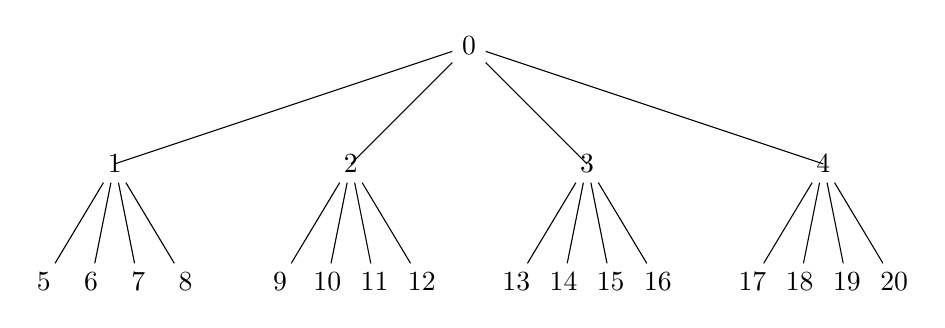
\begin{tikzpicture}
         \node{0}[sibling distance=3cm]
         child{[sibling distance=0.6cm] node{1}
           child{node{5}}
           child{node{6}}
           child{node{7}}
           child{node{8}}
         }
         child{[sibling distance=0.6cm] node{2}
           child{node{9}}
           child{node{10}}
           child{node{11}}
           child{node{12}}
         }
         child{[sibling distance=0.6cm] node{3}
           child{node{13}}
           child{node{14}}
           child{node{15}}
           child{node{16}}
         }
         child{[sibling distance=0.6cm] node{4}
           child{node{17}}
           child{node{18}}
           child{node{19}}
           child{node{20}}
         };
       \end{tikzpicture}

\item To find the parent of a node at $i$, take
  $\lfloor((i-1)/d)\rfloor$.  Some examples from the tree above:
  \begin{align*}
    \id{parent}(8) &=   \lfloor((8-1)/4)\rfloor =
     \lfloor 7/4 \rfloor =     \lfloor 1.75\rfloor =
    1\\
\id{parent}(9) &=   \lfloor((9-1)/4)\rfloor = \lfloor 2\rfloor = 2\\
\id{parent}(10) &=   \lfloor((10-1)/4)\rfloor = \lfloor 9/4 \rfloor = 2
  \end{align*}

   \end{itemize}
   
   \item What is the height of a $d$-ary heap of $n$ elements in terms
     of $n$ and $d$?

     As can be seen by examining the above figure, the maximum number
     of elements that can be stored in a $d$-ary heap of height $h$ is
     \[
\max(n) =  \sum_{i=1}^{h}d^i = \frac{d^{h+1}-1}{d-1}
     \]
     In the above example, $d=4$, $h=2$, giving
     \begin{align*}
       \frac{d^{h+1}-1}{d-1} =  \frac{4^{2+1}-1}{4-1}
       = \frac{64-1}{3}
       = 21
     \end{align*}
     So it checks out.


To find $h$, given $d$ and $n$, we need to find the smallest $h$ such
that the above fraction is greater than or equal to $n$, in other
words,
\begin{align*}
  h &= \min\left\{h : \frac{d^{h+1}-1}{d-1} \geq n\right\}
  \end{align*}
Working with that inequality, we want the smallest $h$ such that
\begin{align*}
   \frac{d^{h+1}-1}{d-1} &\geq n\\
   d^{h+1}-1 &\geq n(d-1)\\
   d^{h+1} &\geq n(d-1) + 1\\
\log_d(   d^{h+1}) &\geq \log_d (n(d -1) + 1)\\
  h+1 &\geq \log_d (n(d-1) + 1)\\
  h &\geq \log_d (n(d -1) + 1)-1\\
\end{align*}
and hence
\begin{align*}
  h &= \lceil\log_d (n(d -1) + 1)-1\rceil
\end{align*}
Let's try that on our example.  With $d=4$ and $n=21$ we get
\begin{align*}
  h &= \lceil\log_d (n(d -1) + 1)-1\rceil\\
   &= \lceil\log_4 ((21)(3)  + 1)-1\rceil\\
   &= \lceil\log_4 (63  + 1)-1\rceil\\
   &= \lceil\log_4 (64)-1\rceil\\
   &= \lceil3-1\rceil\\
   &= 2
\end{align*}
So that works.  With one more item, though, $d=4$ and $n=22$, and we get
\begin{align*}
  h &= \lceil\log_d (n(d -1) + 1)-1\rceil\\
   &= \lceil\log_4 ((22)(3)  + 1)-1\rceil\\
   &= \lceil\log_4 (66  + 1)-1\rceil\\
   &= \lceil\log_4 (67)-1\rceil\\
   &= \lceil3.033-1\rceil\\
   &= 3
\end{align*}
So, yes, with one more item we will need another level in the height
of our tree, which is obvious from the example and so our formula
checks out here, too.




\begin{itemize}
  \item We follow one path from root to leaf, looping over up to $d$
    children at each level, so running time is $O(d\log_d
n)$.  We loop over $d$, but for a $d$-ary heap $d$ is a constant and
does not depend on the input, so the loop is constant for all inputs,
so we could say $O(\log_d n)$
\end{itemize}


     \item Give an efficient implementation of \textsc{Insert} in
       a $d$-ary max-heap.  Analyze its running time in terms of $d$
       and $n$.



       \begin{itemize}\item         
Nothing has to be changed as long as we use the new definition of
\textsc{Parent}.  Time is $O(\log_d n)$.
       \end{itemize}


     \item Give an efficient implementation of
       \textsc{Increase-Key}$(A,i,k)$,
       which flags an error if $k < A[i]$, but otherwise sets $A[i] =
       k$ and then updates the $d$-ary max-heap structure
       appropriately.    Analyze its running time in terms of $d$
       and $n$.



       \begin{itemize}\item         
Nothing has to be changed as long as we use the new definition of
\textsc{Parent}.   Time is $O(\log_d n)$.
       \end{itemize}


\end{description}

\end{document}
